\section{SRAM PUF}

SRAM PUF was first proposed by Guajardo and Holcomb in 2007. SRAM PUF uses existing SRAM blocks to generate chip-specific data.
Normally, when using SRAM to store data, a positive feedback is given to force the cell into one of the two states (a '1' or a '0') available. Once it is there, the cell will be stable and prevented from transitioning out of this state accidentally.
To use it as a PUF, SRAM is turned on and its cell values are retrieved to generate a unique chip-specific output. After powering-up the circuit, the cells stabilize at a state which is defined by the mismatches between the involved transistors. Thus, each SRAM cell provides one bit of output data. To be eligible as a PUF component, an SRAM has to have stable outputs which means any noise has to have little effect on its start-up behavior. In addition, the distribution of 1's and 0's in the SRAM values ideally has to be equal (around 50:50) to ensure there is sufficient amount of randomness exist in the SRAM \cite{6865541}. The distribution of 1's and 0's can also be referred as hamming weight.

As mentioned at the beginning of this chapter, during enrollment, challenge-response pairs are gathered. In SRAM PUF, there are two types of challenges that can be applied to the system. The challenge can be either the whole SRAM memory or specific addresses. If a set of addresses is given as a challenge, an address in there can refer to an address of a byte, a bit, or a sequence of bytes or bits.

\subsection{SRAM Cell}
SRAM uses its SRAM cells to store the binary information. The most common SRAM design is six-transistor (6-T) CMOS SRAM, shown in Figure \ref{fig:sram_cell}. This design utilizes the concept of cross-coupled inverters, constructed by two inverters, each established by two transistors; inverter 1 by Q2 and Q6, inverter 2 by Q1 and Q5. Using this design means the input of an inverter is the output of the other and vice-versa, which also indicates that the output of one inverter is exactly the opposite of the other inverter \cite{modeling_sram}.
Transistors Q3 and Q4, referred as the access transistors, are used as the entry gate to the cell every time a read or write operation will be performed. The bitline (BL), the compliment bitline (BLB) and the wordline (WL) are employed as an entry to the cell. In addition, an SRAM cell will lose its state shortly after power down \cite{maes_2016}.

\begin{figure}[tph!]
    \centerline{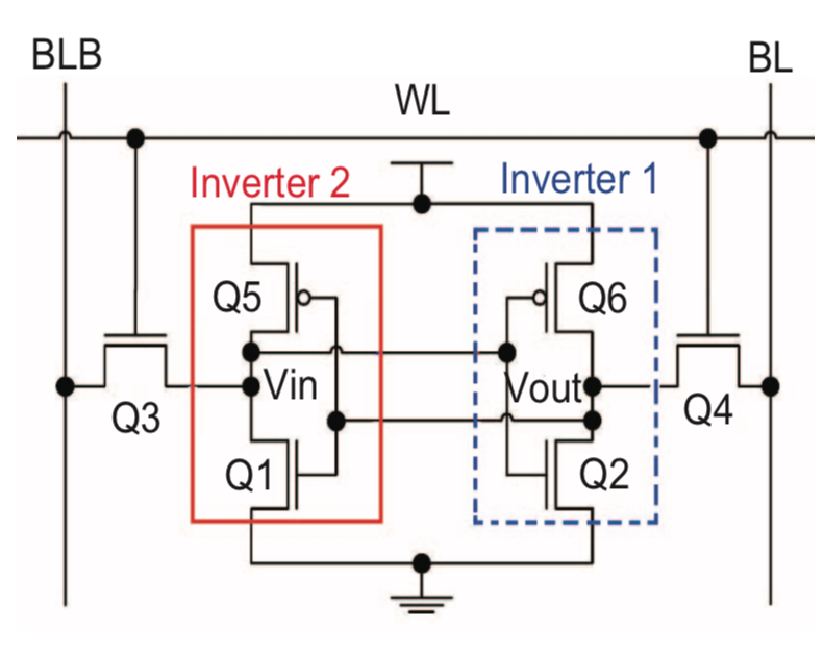
\includegraphics[width={0.5\textwidth}]{images/sram_cell}}
    \caption{A 6-T CMOS SRAM cell \cite{modeling_sram}.}
    \label{fig:sram_cell}
\end{figure}

During manufacturing, there are small differences between each SRAM cell due to process variation which leads to a mismatch in the cell \cite{dargar_2011}. This mismatch also means that the two inverters will always conduct distinctly. Since this mismatch determines the value of the power-up state of an SRAM cell, the power-up state of a cell will be biased towards 0 or 1 depends on the mismatch value. The mismatch itself does not disturb the normal storage functionality of SRAM cell. Based on this bias, SRAM cells can be classified into three categories as shown below:

\begin{enumerate}
\item Non-skewed cell\newline
A non-skewed cell has no preference during its startup due to the impact of process variations does not cause any mismatch between the two inverters. This cell generates bit arbitrarily depending upon the noise introduced in the system.
\item Partially-skewed cell\newline
A partially-skewed cell has a small mismatch between the inverters which lead to a preference over value '0' or '1' but the cell can flip its value upon variation in external parameters.
\item Fully-skewed cell\newline
A fully-skewed cell is a heavily mismatched SRAM cell in a way that the cell inclined towards value '1' or '0' and has a resistance against external influence/noises.
\end{enumerate}


\subsection{Problem: Noise}\label{ch:sram_noise}

Similar to most electronic components, SRAM PUF is also affected by any external influence which leads to noises. These noises will flip unstable bits inside the SRAM PUF. Below are some factors presenting noises:

\begin{itemize}
\item Voltage\newline
The noise introduced by voltage is called power supply noise \cite{wang_tehranipoor_2010}. This noise is related to changes in the delay characteristics of the gate. The changes will occur when there are switchings in the circuit after the device is turned on which increase dynamic power and cause a voltage drop on power lines and voltage increase on ground lines.
\item Temperature\newline
Temperature variation can be introduced by the surroundings or voltage variation. The preference of a cell inside SRAM has a high probability to be affected by temperature.
Temperature affects more than voltage on bit flipping.
\item Crosstalk\newline
Crosstalk appears when a signal transmitted on a circuit introduces unwanted side effects in another circuit. Crosstalk happens due to a tight gap between the SRAM cell (tiny interconnect spacing and width). This event becomes more popular due to wider use of faster-operating speeds and smaller geometries (advancement in nanometer technologies) which lead to higher density. Crosstalk is a major contributor to signal integrity problems in modern designs \cite{wang_tehranipoor_2010}. In addition, higher density in SRAM also influences how environments affect SRAM performance (more prone to voltage and temperature difference) \cite{Abu-Rahma2013}.
\item Aging\newline
Aging is related to changes in the silicon after usage for a long time \cite{rao_mahmoodi_2011}. There are three main effects related to the aging of a circuit; time-dependent dielectric breakdown (TDDB), bias temperature instability (BTI) and hot carrier injection (HCI) \cite{Maricau2013}. TDDB is associated with the creation of a conduction path through the gate transistor structure which causes an increase in power consumption and the circuit delay \cite{impact_mosfet}.
BTI causes a degradation of the transistor threshold voltage \cite{temporal_performance}.
HCI generates a change in the transistor threshold voltage \cite{impact_hot_carriers}. HCI is caused by a high current in the transistor channel injecting charges into the gate oxide during the switching.
\end{itemize}

\subsection{Bit Selection Algorithm} \label{lbl:bit-selection}
Since bit responses are used as the primary input for SRAM PUF, one of the major steps on using SRAM PUF if locations of bits is used as the challenge is looking for stable bits. Stable bits itself refers to fully skewed cells explained before.
Even though the error correction code is present to correct the noise of bit responses, it also has a limitation on how many bits it can correct.
Since not every SRAM cell is stable, one should take a special caution on deciding which SRAM cell is gonna be the bits to use as PUF input.

Choosing the most stable bits is important to ensure that the PUF result is always the same throughout its lifetime.
In here, we use two known algorithms to search for stable bits.

\subsubsection{Neighbor Analysis}
The first algorithm is using the rank of total stable neighbors \cite{xiao_rahman_forte_huang_su_tehranipoor_2014}. They argue that the cells which are “most stable” across environmental conditions are surrounded by more stable cells during enrollment. A stable cell surrounded by more stable cells has a tendency to become more stable because its neighboring cells are likely to experience similar aging stress and operating conditions.
In this algorithm, all the stable cells are given weight according to the number of stable bits surrounding it.
The more stable neighbor cells it has, the higher weight it gets. For example, if a cell is not stable, it is given zero as its score. If it is stable, at least it will get score one. If it only has one stable neighbor on each left and right side, it will get score two as result of an addition of one from being a stable cell and one from having a stable neighbor on both sides. To get score three, it needs to be stable and has two stable neighbors on left and right sides.
After determining the weight of each cell, a heuristic algorithm that greedily chooses cells for the PUF ID/key with weight greater than a threshold is used.

Before the algorithm is performed, one should collect lots of SRAM cells value first. The data should be retrieved in various condition, for example, different voltages, temperatures, and time differences between enrollment.
Afterwards, using the data gathered, the location of all stable bits in SRAM need to be located. A stable bit has to has the same value in all enrollment.
Last, the neighbor analysis algorithm is performed to get the most stable bits in SRAM.

\subsubsection{Data Remanence Approach}

Another bit selection algorithm is by using data remanence of SRAM cell \cite{liu_zhou_tang_parhi_kim_2017}.
There are only two remanence tests involved in this approach: first, writing a value (‘1’ or ‘0’) to the whole memory and second, briefly turning off the power until a few cells flip. The most robust cells are the cells which effortlessly flipped when written with the opposite data. Strong 1's are bits that are flipped fast after 0 is written to its location. On the contrary, if 1 is written to a bit location and the bit flipped fast, it means that the bit is a strong 0.
When using this approach, one should carefully determine the temporal power down time. On one hand, if the temporal power down period is too little, then the data will stay in the previously written state. On the other hand, if the temporal power down time is too lengthy, then the data written in the array will shattered and the SRAM values will go back to its uninitialized state.

A significant advantage using this algorithm compared to the previous one is a much shorter time required to locate stable bits. Using neighbor analysis, there are many SRAM values need to be gathered first which might take hours or days. Locating stable bits from hundreds of data probably also take time as well. If data remanence approach is utilized, there is no need to gather many data. One only need to determine the temporal power down required to get strong bits required. Since usually the temporal down period required is less than 0.5 seconds, this analysis only takes less than one or two minutes.

\section{PUF Applications}

\subsection{Key Generation using SRAM PUF}

In this section, there are two schemes for key generation presented. Both constructions were built by Hyunho Kang et. al. in 2014. The first construction, shown in Figure \ref{fig:cryptographic_key_generation_old}, utilizes random number generator (RNG). This design was perfected in the second design shown in Figure \ref{fig:cryptographic_key_generation}. In the second design, random number generator was removed to make the construction more efficient without affecting the security.
The block length ($n$) of the error correcting code in these schemes is 255.

\begin{figure}[tph!]
    \centerline{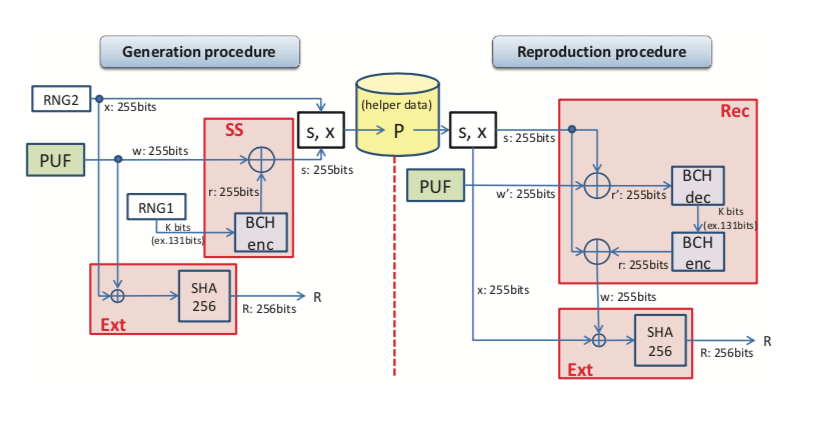
\includegraphics[width={\textwidth}]{images/crypt_key_generation_old}}
    \caption{Implementation diagram using fuzzy extractor (N = 255) \cite{cryptographic_key_generation_old}.}
    \label{fig:cryptographic_key_generation_old}
\end{figure}

\begin{figure}[tph!]
    \centerline{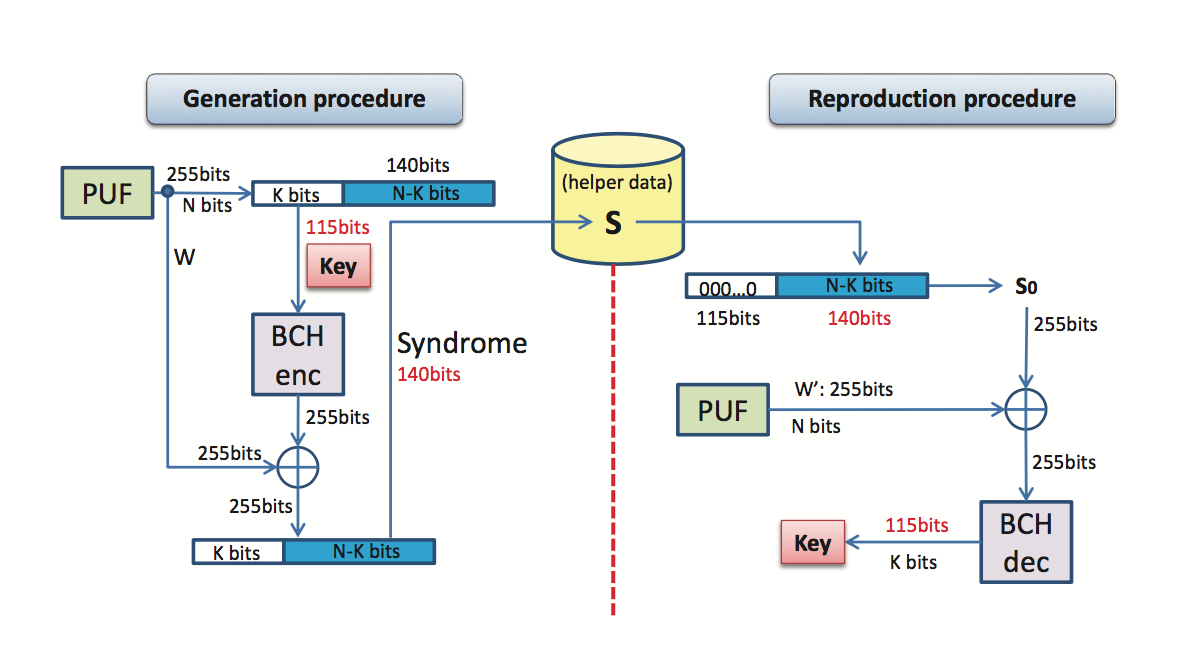
\includegraphics[width={\textwidth}]{images/crypt_key_generation}}
    \caption{Implementation diagram for efficient fuzzy extractor based on the syndrome (N = 255) \cite{cryptographic_key_generation}.}
    \label{fig:cryptographic_key_generation}
\end{figure}

\subsection{Secret Key Binding based on Fuzzy Commitment Scheme}
Fuzzy commitment was originally introduced by Juels and Wattenberg in 1999 \cite{Juels:1999:FCS:319709.319714}. Figure \ref{fig:fuzzy_commitment} shows the flow of this scheme.
To securely bind the secret, the secret key $S^K$ needs to be chosen first. Afterwards, the secret key is encoded into a binary codeword $C^N$. Then, the helper data $M^N$ is generated by masking (\textit{xor}-ing) the codeword with the PUF value $X^N$.
To reconstruct the secret, a noisy version of the codeword $\widetilde{C}^N$ need be calculated by masking the helper data with the noisy version of PUF observation $Y^N$. The secret $\widehat{S}^K$ can be regenerated by decoding the $\widetilde{C}^N$.

\begin{figure}[tph!]
    \centerline{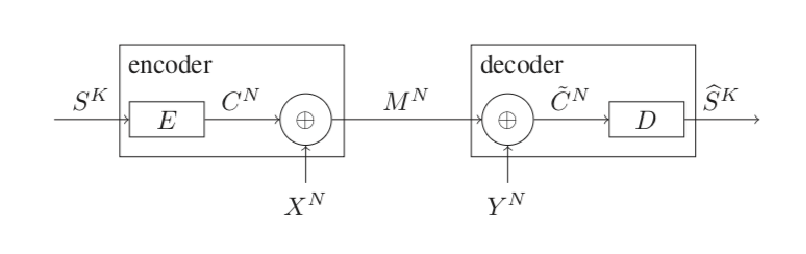
\includegraphics[width={\textwidth}]{images/fuzzy_commitment}}
    \caption{Fuzzy commitment scheme \cite{8006840}.}
    \label{fig:fuzzy_commitment}
\end{figure}


\subsection{Secure Key Storage using Optical PUF and Coating PUF}
In \cite{Skoric2007}, Skoric et. al. present a secure key storage scheme using two extrinsic PUFs; coating PUF and optical PUF. Coating PUF technology is built upon on-chip capacitive quantifications of arbitrary dielectric characteristics of a covering layer which located on top of an IC \cite{10.1007/11894063_29}.  Optical PUF itself consists of a 3-D physical structure containing randomly distributed light-scattering particles that produces a speckle pattern (response) when irradiated with a laser beam \cite{Skoric2007}. This speckle pattern can be considered as the unique fingerprint of the structure. Both PUFs are also considered a strong PUF (has a large CRPs), but optical PUF is considered to be superior than coating PUF due to a much higher number of CRPs and more entropy per response.

% In their scheme, there are two main principle to protect a long term key against physical attacks. First, long term keys should not be stored in non-volatile memory. Second, never let significant portions of the key reside in the volatile memory.
In their scheme, to securely store the key, they proposed to store the long-term key in encrypted form. To access the long-term key, a short-term key extracted from the PUF is required.

\section{Previous Experiments on Off-The-Shelf SRAM PUF}\label{ch:prev_experiments}
There are many experiments related to SRAM PUF which performed on off-the-shelf SRAM. Most of these experiments are using off-the-shelf SRAM that embedded in a microcontroller. For example, in \cite{VanHerrewege:2013:DIP:2541806.2512493}, Herrewege et. al. demonstrate a testing of SRAM characteristics on five different microcontrollers; ARM Cortex-A, ARM Cortex-M, Atmel AVR, Microchip PIC16 and Texas Instruments MSP430. They show that not every SRAM embedded in a microcontroller is ideal for an SRAM PUF such as Microchip PIC16F1825. Fortunately, the other microcontroller's SRAMs show a satisfying result to be a PUF candidate.
Another example is a work done by Anagnostopoulos et. al. \cite{cryptoeprint:2016:769} in which they present low-temperature data remanence attacks against intrinsic SRAM PUFs, specifically ARM Cortex-M4F LM4F120H5QR microcontroller.

Even though not as many as experiments done on microcontroller's SRAM, there are also some related works that doing the experiments using off-the-shelf that is not embedded in a specific device. Akhundov in \cite{haji} presents a concept of using SRAM Microchip 23LC1024 as the root-of-trust of his public-key based authentication architecture. He shows the result of HD\textsubscript{intra}, HD\textsubscript{inter} and the distribution of 0's and 1's experiment of Microchip 23LC1024, and concluded that this SRAM component can be a PUF device. Unfortunately, the testing was not performed in various condition (different voltage, temperature, and aging effect).
Schrijen and van der Leest in \cite{Schrijen:2012:CAS:2492708.2493033} shows a comparative analysis of seven different SRAMs which manufactured using different technology; Cypress \seqsplit{CY7C15632KV18} (65nm),
Virage HP ASAP SP ULP 32-bit (90nm), Virage HP ASAP SP ULP 64-bit (90nm), Faraday \seqsplit{SHGD130-1760X8X1BM1} (130nm), Virage \seqsplit{asdsrsnfs1p1750x8cm16sw0} (130nm), Cypress \seqsplit{CY7C1041CV33-20ZSX} (150nm), and IDT \seqsplit{71V416S15PHI} (180nm). All of them are tested on the reliability (temperature and voltage variance) and uniqueness (HD\textsubscript{inter} and hamming weight). The results between each SRAM type is different but it can be summarized that all of the tested SRAM memories are suitable as a PUF candidate. Another interesting result from these work is the fact that the most reliable SRAM is achieved by IDT 71V416S15PHI followed by Cypress CY7C1041CV33-20ZSX and Cypress CY7C15632KV18.
Another publication is presented by Holcomb et al. \cite{4674345} where they show start-up measurements from ISSI SRAM, TI microcontrollers, and Intel WISP devices. Unfortunately, the manufacturing technology on these devices is not mentioned.
% Another example is a work done by Zhang et.al in \cite{7459321} where they did an experiment of introducing a novel PUF implementation of the second category that exploits the effect of manufacturing process variations in SRAM read access current
% on SRAM ISSI IS62C256AL to explot Current based PUF Exploiting Random Variations in SRAM Cells
